\documentclass{beamer}
\usepackage{graphicx}
\usepackage{xcolor}
\usepackage{tikz}

% 自定义颜色
\definecolor{purpleblue}{RGB}{80, 80, 180}
\definecolor{lightgray}{RGB}{230, 230, 230}
\definecolor{novelPurple}{RGB}{98, 54, 255} 
\definecolor{darkgray}{RGB}{50, 50, 50}

% 主题设置
\usetheme{Madrid}  
\usecolortheme{dolphin} 

% 设置字体（移除 fontspec，确保 pdfLaTeX 兼容）
\setbeamerfont{title}{size=\Large,series=\bfseries}
\setbeamerfont{frametitle}{size=\LARGE,series=\bfseries}
\setbeamercolor{frametitle}{fg=white, bg=novelPurple}
\setbeamercolor{title}{fg=white, bg=purpleblue}

% 封面信息
\title[SAT Hard Question]{\textbf{SAT Hard Question 15}}
\author{\textbf{Jack Zeng}}
\institute{\textcolor{white}{\textbf{Novel Prep}}}
\date{\today} 

\begin{document}

% --- Title Slide ---
\begin{frame}
    \titlepage
    \vfill
    \begin{flushright}
        \textcolor{purpleblue}{\Huge \textbf{Novel Prep}}
    \end{flushright}
\end{frame}


\begin{frame}
    \begin{tikzpicture}[remember picture, overlay]
        % 设置浅色渐变背景
        \shade[top color=softPurple, bottom color=softGray] 
            (current page.north west) rectangle (current page.south east);
        
        % 添加高斯模糊光晕
        \fill[white, opacity=0.3] (current page.center) circle (4cm);
        
        % 主标题
        \node[align=center] at (current page.center) {
            {\Huge\bfseries\textcolor{purpleblue}{Novel Prep}} \\[0.5cm]
            {\Large\itshape\textcolor{lightText}{Excellence in SAT Prep}}
        };

        % 添加柔和光点（点缀）
        \foreach \x in {1,2,3,4,5} {
            \fill[purpleblue, opacity=0.2] (rand*10-5, rand*7-3.5) circle (0.1+\x*0.05);
        }

        ;
    \end{tikzpicture}
\end{frame}

\begin{frame}{Question: Quadratic Function}
\textbf{Which of the following ensures that the Quadratic  equation}  
\[
ax^2 - 4x + c = 0
\]  
\textbf{has at least one real root?}

\vspace{1em}

\begin{enumerate}
\item[A] \(a > 0\)
\item[B] \(a = 0\)
\item[C] \(c > 0\)
\item[D] \(c = 0\)
\end{enumerate}
\end{frame}
\begin{frame}{Answer}

Answer: D
    
\end{frame}


\begin{frame}{Question }
\small
\begin{center}
    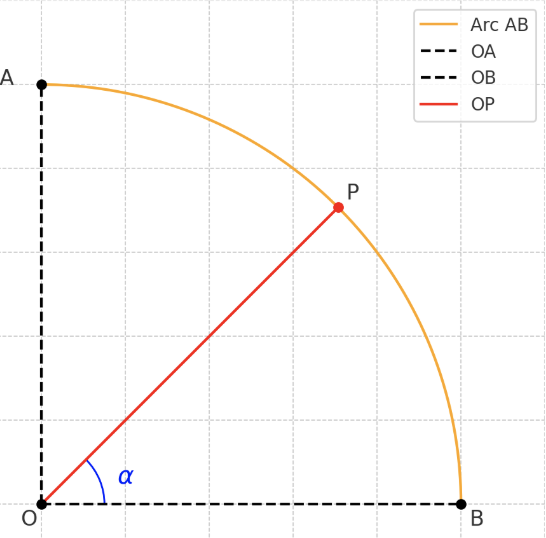
\includegraphics[width=0.3\linewidth]{f11.png}
\end{center}
\textbf{As shown in the figure, \(O\) is the center of a circle with radius 1, and the circle intersects the coordinate axes at points \(A\) and \(B\).  
Point \(P\) lies on arc \(\overset{\frown}{AB}\) (not overlapping with \(A\) or \(B\)). Connect \(OP\), and let \(\angle POB = \alpha\).  
What are the coordinates of point \(P\)?}




\begin{enumerate}
\item[A] \((\sin\alpha, \sin\alpha)\)
\item[B] \((\cos\alpha, \cos\alpha)\)
\item[C] \((\cos\alpha, \sin\alpha)\)
\item[D] \((\sin\alpha, \cos\alpha)\)
\end{enumerate}
\end{frame}

\begin{frame}{Answer}

Answer: C
    
\end{frame}



\begin{frame}{Question: Stats}
\textbf{The following table shows the age distribution of a school choir's members:}

\vspace{1em}
\begin{center}
    

\begin{tabular}{|c|c|c|c|c|}
\hline
\textbf{Age (years)} & 13 & 14 & 15 & 16 \\
\hline
\textbf{Frequency} & 5 & 15 & \(x\) & \(10 - x\) \\
\hline
\end{tabular}
\end{center}

\vspace{1em}

\textbf{For different values of \(x\), which pair of statistical measures regarding age will not change?}

\vspace{1em}

\begin{enumerate}
\item[A] Mean, Median  
\item[B] Mode, Median  
\item[C] Mean, Standard Deviation  
\item[D] Median, Standard Deviation
\end{enumerate}

\end{frame}

\begin{frame}{Answer}

Answer: B
    
\end{frame}

\begin{frame}{Question }
\textbf{Given that the line \(y = kx + k + 1\) passes through the points \((m, n + 3)\) and \((m + 1, 2n - 1)\), and that \(0 < k < 2\), what is a possible value of \(n\)?}

\vspace{1em}

\begin{enumerate}
\item[A] 3
\item[B] 4
\item[C] 5
\item[D] 6
\end{enumerate}

\end{frame}

\begin{frame}{Question }
\textbf{The graph of the quadratic function \(y = |a| x^2 + bx + c\) passes through the following five points:}  
\[
A(m, n), \quad B(0, y_1), \quad C(3 - m, n), \quad D(\sqrt{2}, y_2), \quad E(2, y_3)
\]  
\textbf{What is the correct order of \(y_1, y_2, y_3\)?}

\vspace{1em}

\begin{enumerate}
\item[A] \(y_1 < y_2 < y_3\)
\item[B] \(y_1 < y_3 < y_2\)
\item[C] \(y_3 < y_2 < y_1\)
\item[D] \(y_2 < y_3 < y_1\)
\end{enumerate}

\end{frame}

\begin{frame}{Question}

\begin{center}
    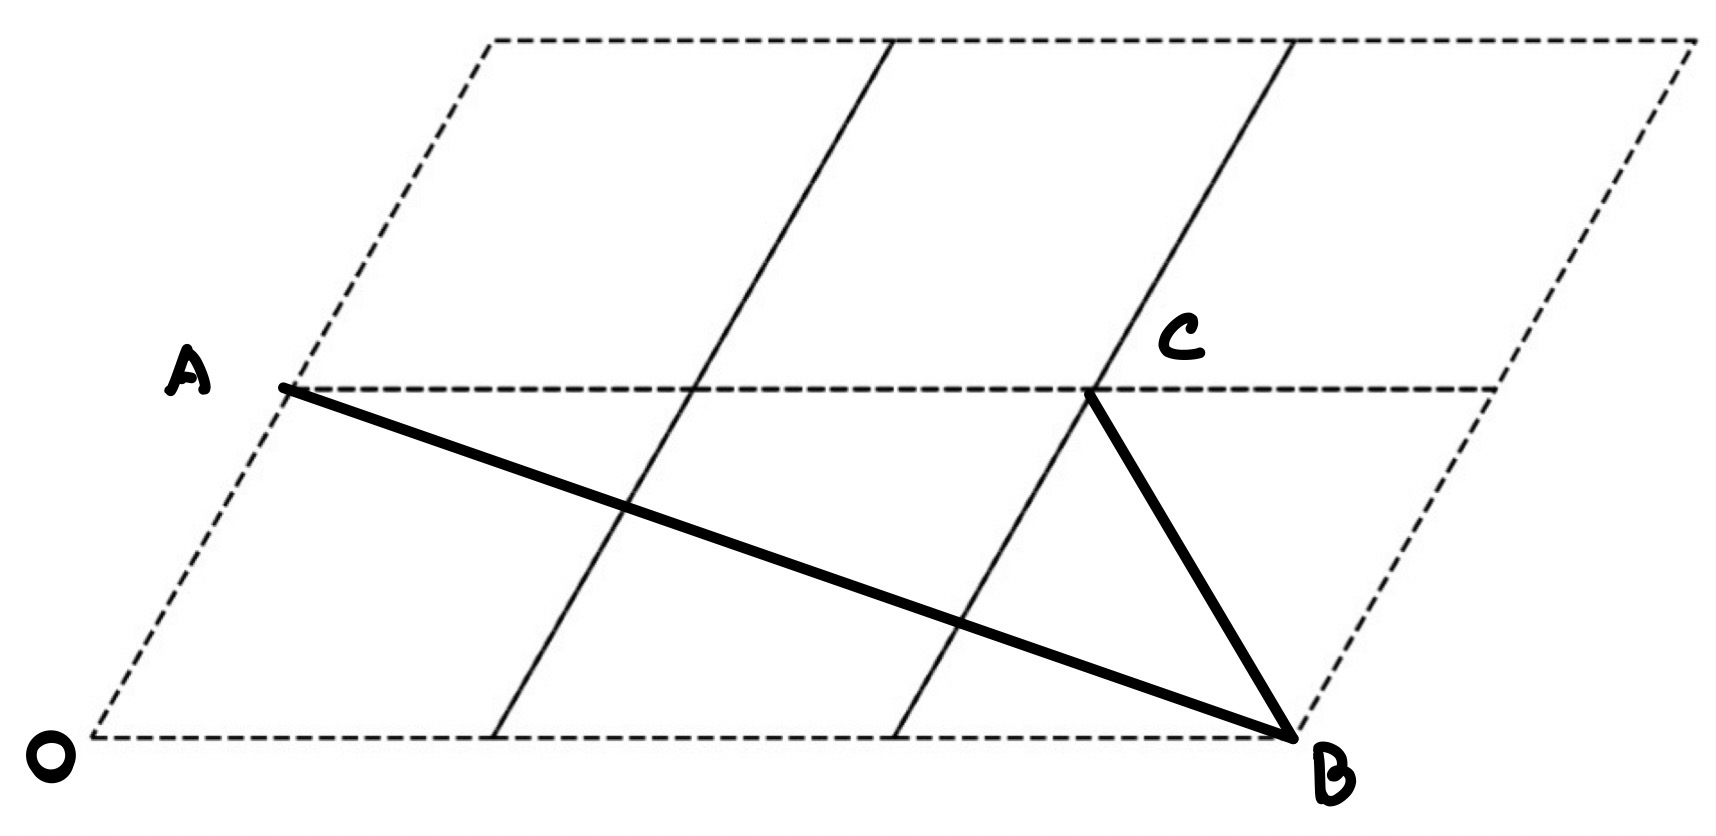
\includegraphics[width=8cm\linewidth]{f12.jpg}
\end{center}
As shown in the figure, 6 identical rhombuses form a grid. The vertices of the rhombuses are called grid points.  
It is known that one angle of the rhombus, $\angle O$, is $60^\circ$, and points $A$, $B$, and $C$ are located on grid points.  
Find the value of $\tan \angle ABC$.


\end{frame}


\begin{frame}{Question 10: Quadratic Function Reasoning}

\textbf{Given} the quadratic function  
\[
y = x^2 - 2ax + a \quad (a \ne 0)
\]  
passes through two points  
\[
A\left( \frac{a}{2}, y_1 \right), \quad B(3a, y_2),
\]  
which of the following statements is correct?

\vspace{1em}
\begin{enumerate}[A.]
    \item There exists a real number \( a \) such that \( y_1 > a \).
    \item For all real numbers \( a \), \( y_1 > a \) is always true.
    \item There exists a real number \( a \) such that \( y_2 < 0 \).
    \item For all real numbers \( a \), \( y_2 < 0 \) is always true.
\end{enumerate}

\end{frame}

\begin{frame}{Question}
As shown in the figure, in triangle \(\triangle ABC\), \(\angle BAC = 90^\circ\), \(AB = AC\),  
Circle \(O\) has diameter \(AB\), and intersects \(BC\) at point \(D\).  
Line \(AE \perp OC\), with foot of the perpendicular at point \(E\).  
The extension of line \(BE\) intersects \(AD\) at point \(F\).

\vspace{1em}
\item Find the value of \(\dfrac{OE}{AE}\).


\begin{center}
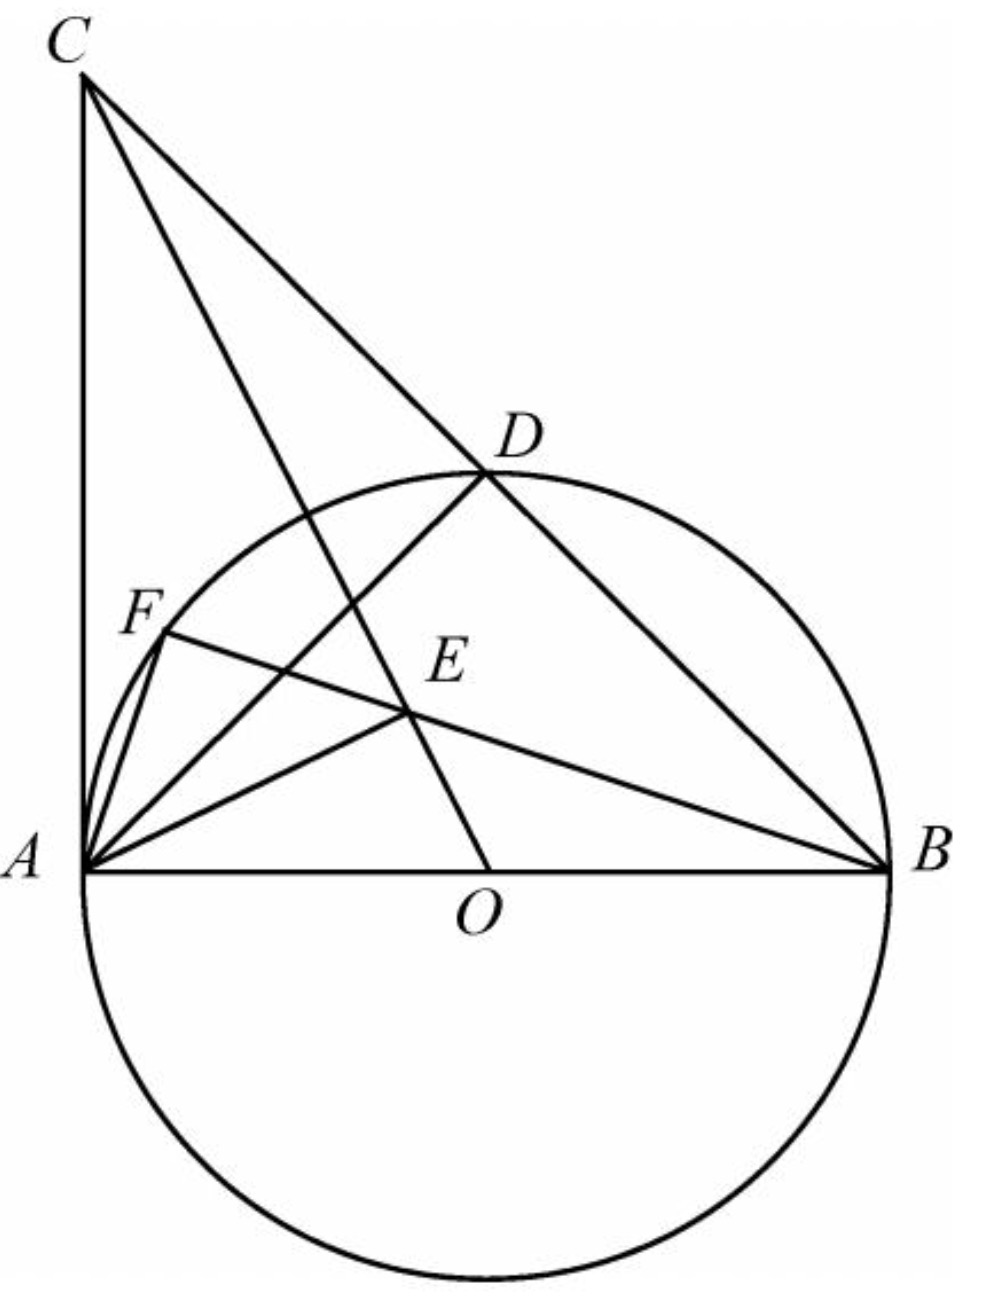
\includegraphics[width=0.29\textwidth]{f14.jpg} % Replace with actual image in your Overleaf or local setup
\end{center}
\end{frame}

\begin{frame}{Answer}

1/2
    
\end{frame}

\begin{frame}{Question}


In rectangle $ABCD$, point $B$ is the center of a circle $\odot B$ with radius $BC$. The circle intersects $AB$ at point $F$. Point $E$ lies on $AD$, and segment $CE$ is rotated about $E$ to form $EG$ such that point $G$ lies on $\odot B$, where $\angle GEC = 90\degree$. Point $F$ is the midpoint of $EG$. Given that $AF = 1$, $AE = 3$, find the length of $CD = \underline{\hspace{2cm}}$.
\begin{center}
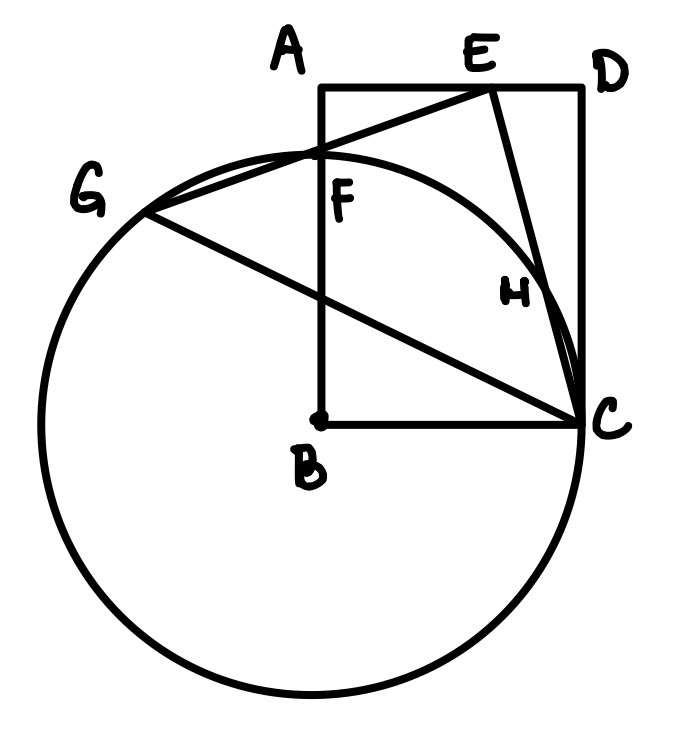
\includegraphics[width =0.4\linewidth]{f15.jpg}
\end{center}




\end{frame}







\end{document}
